\section{Homework 1}

\begin{mdframed}
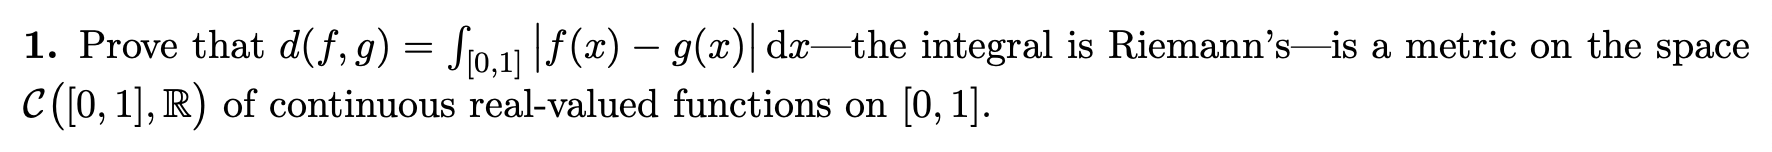
\includegraphics[width=400pt]{img/analysis--berkeley-202a--homework-1-a75a.png}
\end{mdframed}


\begin{proof}
  $d$ is a metric if it satisfies (I) $d(f,f) = 0$, (II) $d(f,g) = d(g, f)$, and (III) $d(f,g) + d(g, h) \le d(f, h)$.

  (I) is satisfied: $d(f, f) = \int_{[0,1]}|f(x) - f(x)| \dx = 0$.

  (II) is satisfied:
\begin{align*}
  d(f, g)
  &= \int_{[0,1]}|f(x) - g(x)| \dx \\
  &= \int_{[0,1]}|g(x) - f(x)| \dx \\
  &= d(g, f),
\end{align*}

  (III) is satisfied:
\begin{align*}
  d(f, g) + d(g, h)
  &= \int_{[0,1]} |f(x) - g(x)| \dx + \int_{[0,1]} |g(x) - h(x)| \dx \\
  &= \int_{[0,1]} |f(x) - g(x)| + |g(x) - h(x)| \dx \\
  &\le \int_{[0,1]} |f(x) - g(x) + g(x) - h(x)| \dx \\
  &= \int_{[0,1]} |f(x) - h(x)| \dx \\
  &= d(f, h).
\end{align*}
\end{proof}

\newpage
\begin{mdframed}
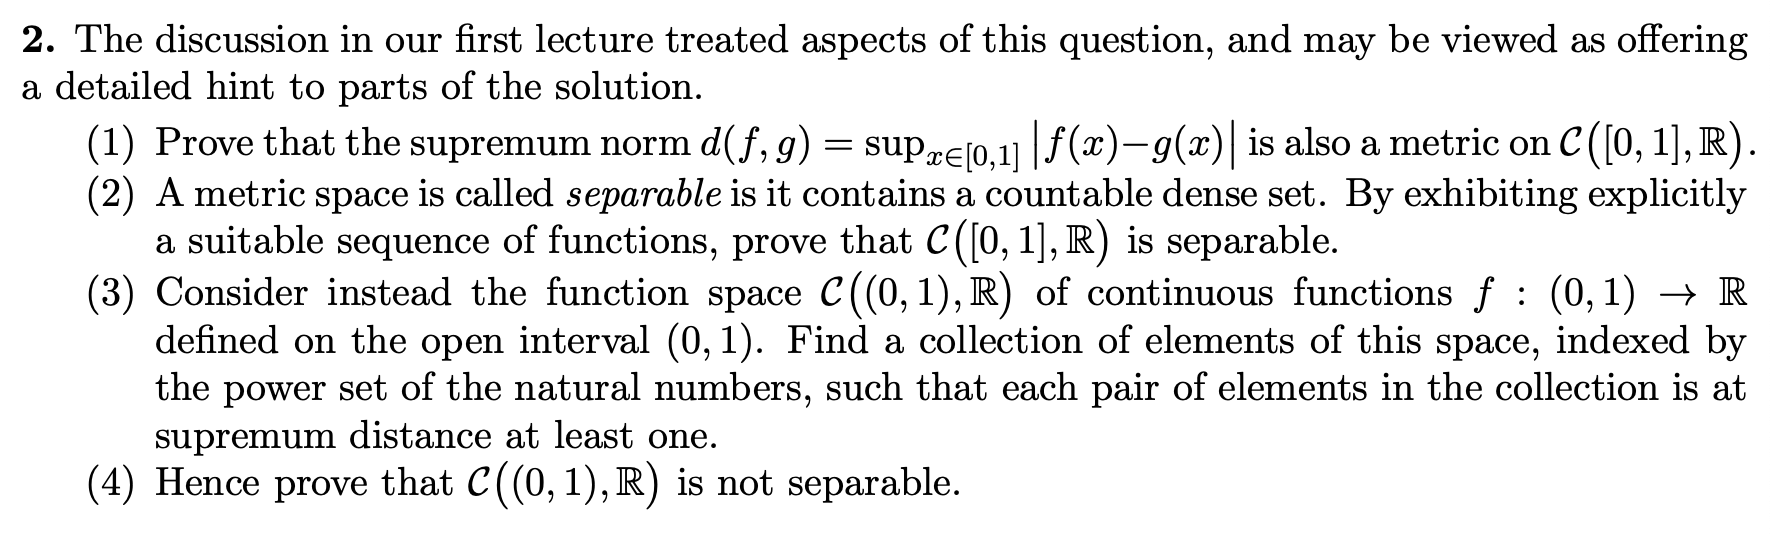
\includegraphics[width=400pt]{img/analysis--berkeley-202a--homework-1-d1d3.png}
\end{mdframed}


Stone-Weierstrass is relevant but not needed
Weierstrass approximation theorem

Ideally the functions should be bounded. e.g. [0,1] -> [0,1]

sin worth looking at

look for functions where all pairs distance exactly 1

\begin{enumerate}[label=(2.\arabic*)]
\item
  \begin{proof}
    $d$ is a metric on the function space $\mathcal C\([0, 1], \R\)$ if it satisfies (I) $d(f,f) = 0$,
    (II) $d(f,g) = d(g, f)$, and (III) $d(f,g) + d(g, h) \le d(f, h)$.

  (I) is satisfied: $\sup_{x\in [0,1]} |f(x) - f(x)| = \sup_{x\in [0,1]} 0 = 0$.

  (II) is satisfied:
\begin{align*}
  d(f, g)
  &= \sup_{x \in [0,1]}|f(x) - g(x)| \\
  &= \sup_{x \in [0,1]}|g(x) - f(x)| \\
  &= d(g, f),
\end{align*}
  (III) is satisfied:
\begin{align*}
  d(f, g) + d(g, h)
  &=   \sup_{x \in [0,1]} |f(x) - g(x)| + \sup_{x \in [0,1]} |g(x) - h(x)| \\
  &=   \sup_{x \in [0,1]} \Big(|f(x) - g(x)| + |g(x) - h(x)|\Big) \\
  &\le \sup_{x \in [0,1]} |f(x) - h(x)| \\
  &=   d(f, h).
\end{align*}
  \end{proof}

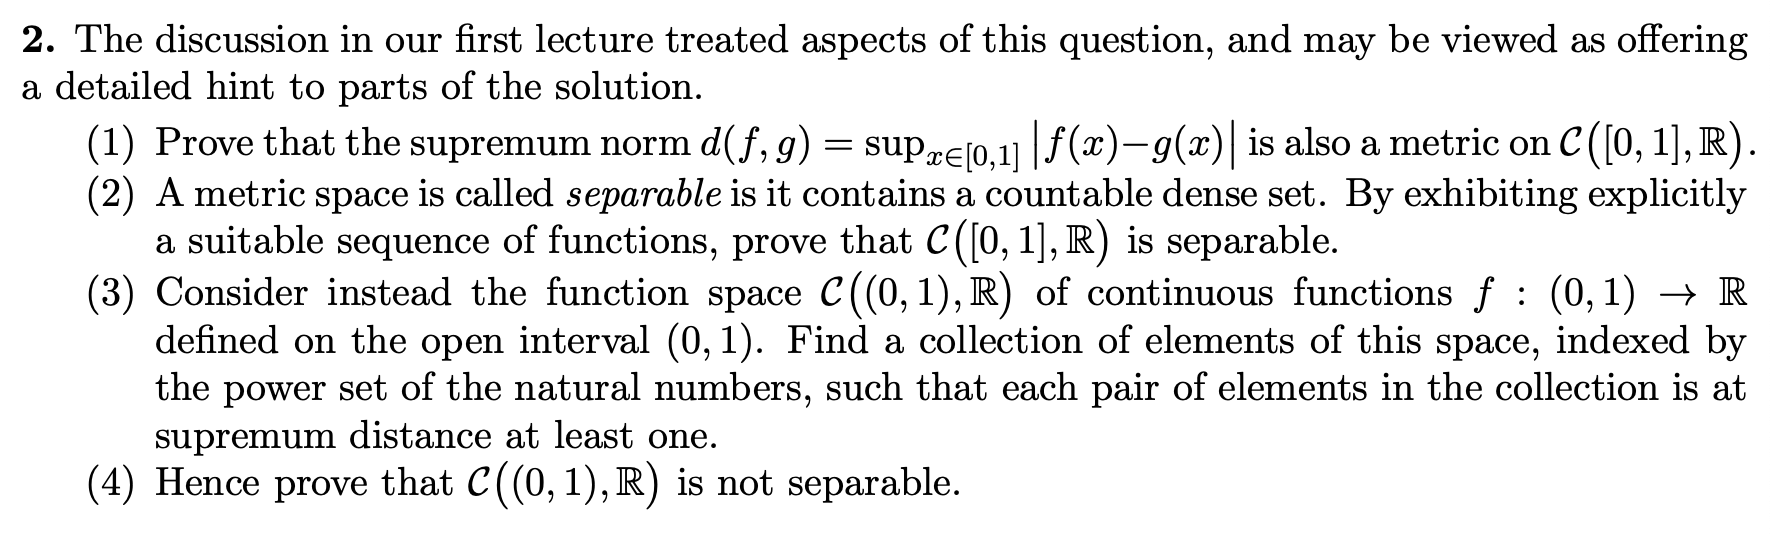
\includegraphics[width=400pt]{img/analysis--berkeley-202a--homework-1-d1d3.png}

\item
  \begin{claim}
    $\mc C\([0, 1], \R\)$ is separable.
  \end{claim}

  \begin{proof}
    Let $\mc G\([0, 1], \R\)$ be the set of piecewise affine functions. Precisely, for all $N \in \N$, for
    all $\x = (x_1, x_1, \ldots, x_{N-1}) \in \Q^{N-2}$, and for all $\y = (y_1, y_2, \ldots, y_N) \in \Q^N$ we
    define $g_{(N, \x, \y)}: [0, 1] \to \R$ to be the function whose graph is drawn by connecting with straight
    lines the sequence of points $(0, y_0), (x_1, y_1), \ldots, (x_{N-1}, y_{N-1}), (1, y_N)$. We will call
    these points the ``grid points​'' of $g$.

    Note that $\Q^{N-2}$ and $\Q^N$ are both countable, since they are finite products of a countable set $\Q$.
    And therefore $\mc G$ is countable, since it is a product of 3 countable sets.

    It remains to show that $\mc G$ is dense in $\mc C\([0, 1], \R\)$. To do so we must show that an
    arbitrary function $f \in \mc C$ can be approximated by a function $g \in \mc G$ in the sense
    that, under the supremum norm $d(\cdot, \cdot)$, for any $\epsilon > 0$ there exists $g \in \mc G$
    such that $d(g, f) < \epsilon$.

    So fix some $f \in \mc C$ and fix some $\epsilon > 0$.

    First we show that there exists a $g$ that approximates $f$ at arbitrarily many points.

    Fix $N \in \N$ and fix a sequence $(\om_1, \om_2, \ldots, \om_{N-1}) \in \R^{N-2}$ such that $\omega_1 < \omega2 < \cdots < \om_{N-1}$.

    Now construct $g \in \mc G$ according to the following procedure:
    \begin{enumerate}
    \item Pick $y_0 \in \Q$ such that $|y_0 - f(0)| < \epsilon$.
    \item Extend a straight line from $(0, y_0)$ through $(\om_1, f(\om_1))$
    \item Pick $(x_1, y_1) \in \Q^2$ such that $\om_1 < x_1 < \om_2$
    \item \red{TODO}
    \end{enumerate}


    Since $[0, 1]$ is compact, $f$ is uniformly continuous.

    Let $g_n \in \mc G$ be the approximating function using a grid spacing of $1/n$.

    $f$ can be approximated at an arbitrary set of finitely many points using the procedure above. I.e. for
    any $\epsilon$ there exists an $n$ such that $|g_n(\om_i) - f(\om_i)| < \eps$ for finitely many points $w_i$.

    We want to show that $f$ is adequately approximated everywhere.

    Let $\omega$ be an arbitrary point not in the set $\{w_i: i \in 1, 2, \ldots, n\}$ used to construct the
    approximation $g_n$.



    Suppose for a contradiction that it is not. Then there exists a $\om \in [0, 1]$ such
    that $|g_n(\om) - f(\om)| \geq \epsilon$ for all $n \in \N$.





    Define $d(f, g)$ to be the supremum distance between functions $f: [0,1] \to \R$ and $g [0,1] \to \R$.

    Let $g$ be an arbitrary function in $\mc C\([0, 1], \R\) \setminus \mc F$ and fix $\epsilon > 0$.
    We need to show that there exists $f \in \mc F$ such that $d(f, g) < \epsilon$. We construct such
    an $f$ using the following algorithm:

    \red{I think the basic idea here is to use the fact that the interval is closed and therefore the target
      function has extrema, so keep drawing lines to the extrema and subdividing; something like that}

    \begin{enumerate}
    \item Set $f$ equal to the function whose graph is a straight line joining $(0, g(0))$ and $(1, g(1))$. In
      other words, set $f$ such that $f(x) = xg(0) + (1-x)g(1)$.
    \item If $d(f, g) < \epsilon$, stop.
    \item Otherwise, divide the interval in half, and repeat the approximation in each half.
    \end{enumerate}
    We need to show that this algorithm terminates.


  \end{proof}

  We must exhibit a sequence of functions that is a dense and countable subset of $\mc C\([0, 1], \R\)$
  under the supremum norm.

  This means that for an arbitrary continuous function $g$, and for any $\epsilon > 0$, we must be able to
  construct a function that lies within $\epsilon$ of $g$.

  \url{https://en.wikipedia.org/wiki/Piecewise_linear_function}

  \begin{quote}
    A piecewise linear function is a function defined on a (possibly unbounded) interval of real numbers,
    such that there is a collection of intervals on each of which the function is an affine function. If the
    domain of the function is compact, there needs to be a finite collection of such intervals; if the domain
    is not compact, it may either be required to be finite or to be locally finite in the reals.
  \end{quote}

  \begin{definition}
    A subset $X$ of a metric space is \defn{open} if for any point $x \in X$, there exists $\epsilon$ such that a ball
    of radius $\epsilon$ centred at $x$ is a subset of $X$.

    A subset $X$ of a metric space is \defn{closed} if it is the complement of an open subset of $X$.

    (Theorem: a set $X^C$ is closed iff it contains all its limit points, i.e. every convergent sequence
    in $X^C$ has its limit in $X^C$.)

    A subset $X$ of a metric space $Y$ is \defn{dense} if every point $y \in Y$ is either in $X$ or arbitrarily close to
    a point in $X$.
  \end{definition}

\item Let $f_S: (0, 1) \to \R$ be given by $f_S(x) = \frac{1}{r(S)x}$, where $S \in 2^\N$ and $r(S) \in [0, 1]$ is
  the real number corresponding to $S$, i.e. the number $r(S) = 0.d_1d_2d_3\ldots$ where
  \begin{align*}
    d_i =
    \begin{cases}
      1, ~~~~ \text{if} ~~~~ i \in S,\\
      0, ~~~~ \text{otherwise}.
    \end{cases}
  \end{align*}
  ... but the supremum distance does not exist for a pair of functions from this set: their difference is
  unbounded.

\item Let $\mathcal F$ be the uncountable collection of functions identified in part (3). Suppose for a
  contradiction that $\mathcal C\([0, 1], \R\)$ is separable. Then it contains a countable dense
  set $\mathcal G$.

\end{enumerate}


\newpage
\begin{mdframed}
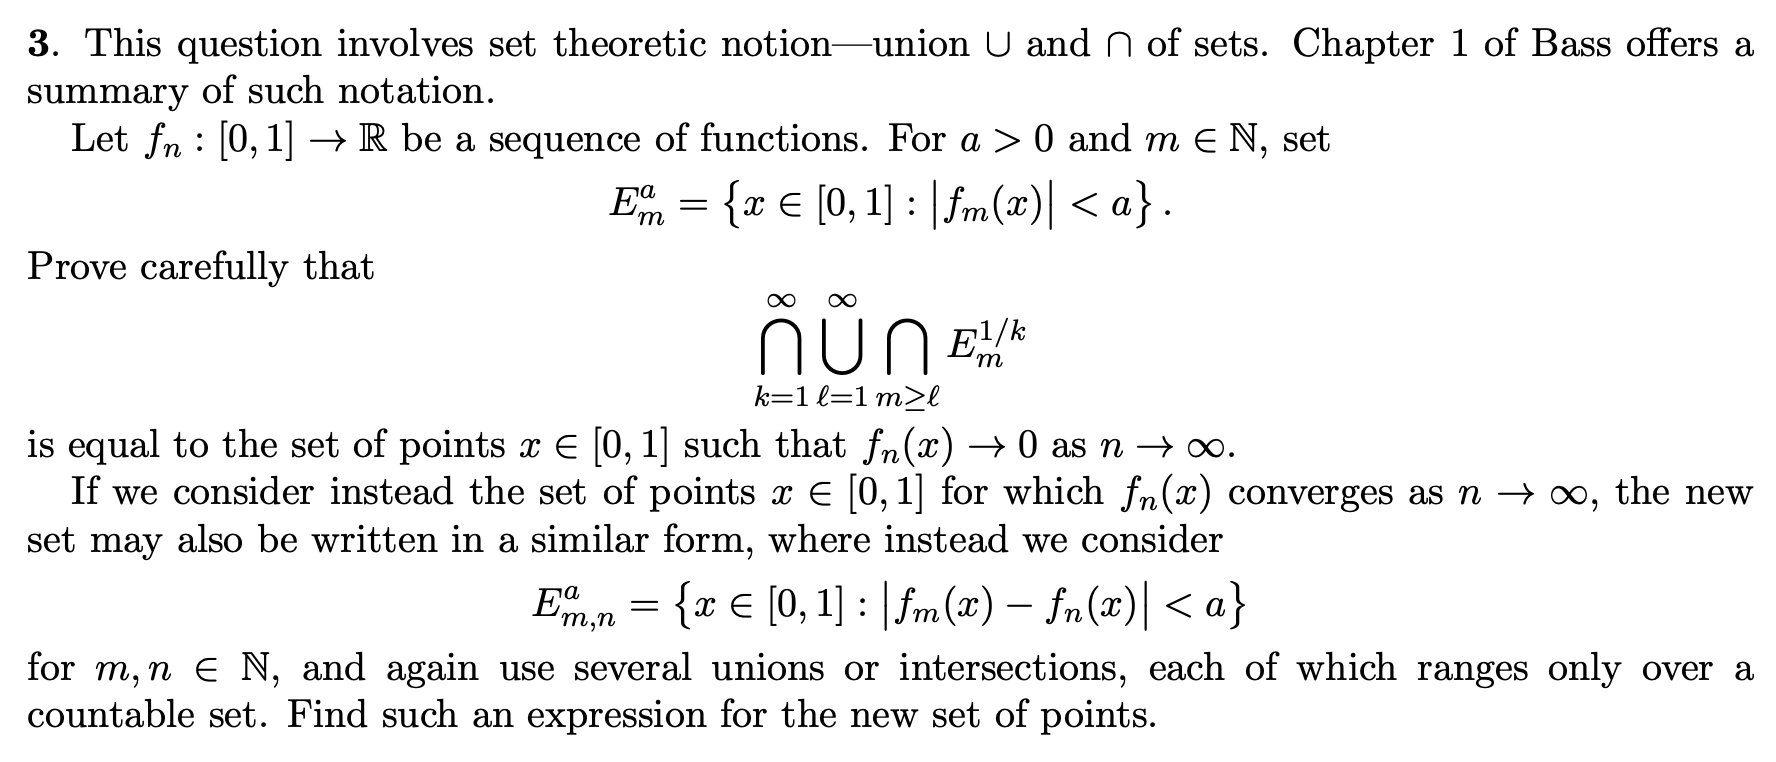
\includegraphics[width=400pt]{img/analysis--berkeley-202a--homework-1-8349.png}
\end{mdframed}


\begin{proof}
  Let $E_m^a = \{x \in [0, 1] : |f_m(x) < a|\}$ and let $T = \bigcap_{k=1}^\infty \bigcup_{l=1}^\infty \bigcap_{m > l} E_m^{1/k}$.

  Informally, $E_m^a$ is the set of points for which $f_m$ is within $a$ of zero.

  Let $f_n: [0, 1] \to \R$ be a sequence of functions and let $S \subseteq [0, 1]$ be the set of points $x$
  such that $f_n(x) \to 0$ as $n \to \infty$.

  First we prove that $x \in S \implies x \in T$.

  So let $x \in S$. Then from the definition of limit we have
  \begin{align*}
    &\forall \epsilon>0 ~~~~ \exists l \in \N ~~~~ \forall m \geq l ~~~~  x \in E_m^\epsilon \\
    \iff &\forall \epsilon>0 ~~~~ \exists l \in \N ~~~~                        x \in \bigcap_{m \geq l} E_m^\epsilon \\
    \iff &\forall \epsilon>0 ~~~~                                              x \in \bigcup_{l=1}^\infty \bigcap_{m \geq l} E_m^\epsilon \\
    \iff &                                                              x \in \bigcap_{k=1}^\infty \bigcup_{l=1}^\infty \bigcap_{m \geq l} E_m^{1/k} = T,
  \end{align*}
  as required.

  Secondly we prove that $x \in T \implies x \in S$.

  So let $x \in T$. We have
  \begin{align*}
    x \in \bigcap_{k=1}^\infty \bigcup_{l=1}^\infty \bigcap_{m \geq l} E_m^{1/k},
  \end{align*}
  which is equivalent to the statement
  \begin{align*}
    \forall k>0 ~~~~ \exists l \in \N ~~~~ \forall m \geq l ~~~~  |f_m(x)| < \frac{1}{k}.
  \end{align*}
  Let $\epsilon > 0$ be a real number. Then there exists $k \in \N$ such that $\frac{1}{k} < \epsilon$. Therefore we have
  \begin{align*}
    \forall \epsilon>0 ~~~~ \exists l \in \N ~~~~ \forall m \geq l ~~~~  |f_m(x)| < \epsilon
  \end{align*}
  which is equivalent to $x \in S$, as required.
\end{proof}

\begin{proof}
  Let $S \subseteq [0, 1]$ be the set of points $x$ for which $f_n(x)$ converges as $n \to \infty$. Since every
  convergent sequence in the reals is Cauchy, we have that $x \in S$ is equivalent to
  \begin{align*}
    \forall \epsilon > 0 ~~~~ \exists l \in \N ~~~~ \forall m \geq l ~~~~ \forall n \geq l ~~~~ |f_m(x) - f_n(x)| < \epsilon,
  \end{align*}
  which is equivalent to
  \begin{align*}
    \forall \epsilon > 0 ~~~~ x \in \bigcup_{l=1}^\infty \bigcap_{m \geq l} \bigcap_{n \geq l} E_{m,n}^\epsilon.
  \end{align*}
  Therefore, we have that $x \in S$ implies
  \begin{align*}
    x \in \bigcap_{k=1}^\infty \bigcup_{l=1}^\infty \bigcap_{m \geq l} \bigcap_{n \geq l} E_{m,n}^{1/k}.
  \end{align*}
  As before, the reverse implication also holds since, for any given $\epsilon > 0$, we can find a $k \in \N$
  such that $\frac{1}{k} < \epsilon$.
\end{proof}

\newpage
\begin{mdframed}
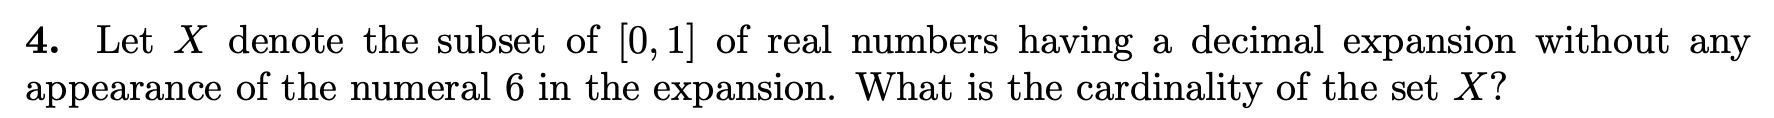
\includegraphics[width=400pt]{img/analysis--berkeley-202a--homework-1-f175.png}
\end{mdframed}


\begin{proof}
  Let $X \subset [0, 1]$ be the subset of real numbers without any 6 in their decimal expansion. Let $x \in X$ and let
  \begin{align*}
    d_n(x) =
    \begin{cases}
      0, ~~~~ n\text{-th decimal place of }x \text{ is }0\\
      1, ~~~~ \text{otherwise}.
    \end{cases}
  \end{align*}
  Thus we see that there is an non-injective surjection from $X$ to the reals in $[0, 1]$ and therefore that
  the cardinality of $X$ is at least that of the reals. Since $X \subset \R$ we conclude that the cardinality
  of $X$ is equal to that of the reals.
\end{proof}

\newpage
\begin{mdframed}
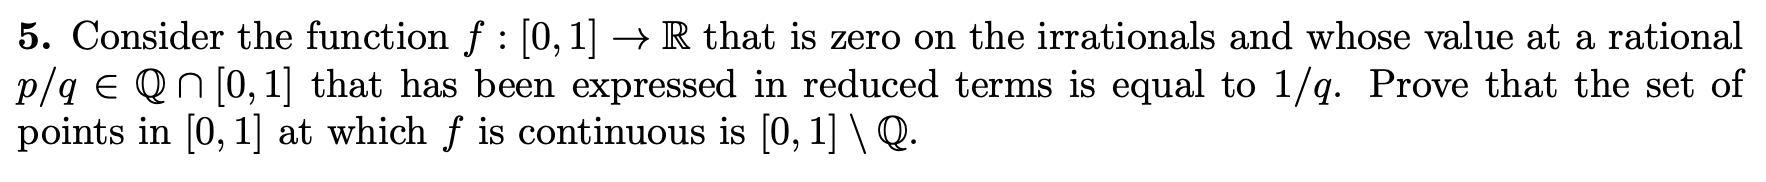
\includegraphics[width=400pt]{img/analysis--berkeley-202a--homework-1-5192.png}
\end{mdframed}



\begin{proof}
  Let $X \subseteq [0, 1]$ be the set of points at which $f$ is continuous. We want to show that $f$ is
  continuous at $x$ iff $x$ is not rational.

  Suppose for a contradiction that $f$ is continuous at a rational point $x = p/q$, where $p, q$ are
  non-negative integers. Then $f(x) = 1/q$. But there will always be irrational points within a given
  distance $\delta$ of $x$, now matter how small $\delta$ is, and at such an irrational point $x'$ we
  have $|f(x) - f(x')| = |1/q - 0| = 1/q$. Therefore $f$ is not continuous at $x$ since the definition of
  continuity does not hold for $\epsilon < 1/q$.

  Now let $x$ be irrational, so that $f(x) = 0$. Fix an arbitrary $\epsilon > 0$. We want to show that there
  exists a $\delta$ such that $1/q < \epsilon$ for any rational point $p/q$ lying within $\delta$ of $x$,
  where $p/q$ is in reduced terms. If $\epsilon > 1/2$ then any $\delta$ will work, so
  assume $\epsilon \leq 1/2$. Let $k$ be the largest natural number such that $1/k \geq \epsilon$, let $i$ be
  the largest natural number such that $i/k < x$ and let $j$ be the smallest natural number such
  that $j/k > x$. Then a choice of $\delta = \frac{1}{2}\min\{x - i/k, j/k - x\}$ will work to prove continuity
  of $f$ at irrational $x$.
\end{proof}

\newpage
\begin{mdframed}
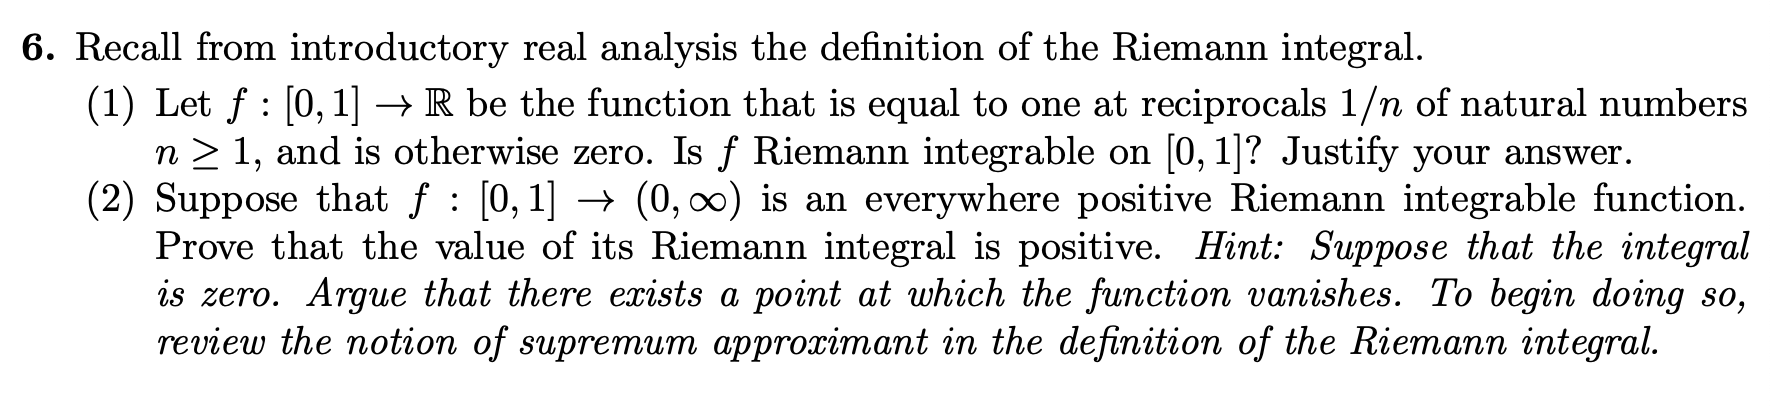
\includegraphics[width=400pt]{img/analysis--berkeley-202a--homework-1-f5e8.png}
\end{mdframed}


\begin{definition}
  $g: [0, 1] \to \R$ is Riemann integrable if
  \begin{align*}
    \sup_{\phi^-} I(\phi^-) = \inf_{\phi^+} I(\phi^+).
  \end{align*}
  Here $\phi^-$ and $\phi^+$ are step functions adapted​ to some
  partition $0 \leq x_1 \leq x_2 \leq \ldots \leq x_{n-1} \leq 1$, such that $\phi(x) = c_i$
  for $x \in (x_{i-1}, x_i)$. $I(\phi)$ is (informally) the area under the step function $\phi$:
  \begin{align*}
    I(\phi) = \sum_{i=1}^n c_i(x_i - x_{i-1}).
  \end{align*}
  And the supremum is over all minorants $\phi^- \leq g$ and the infimum is over all
  majorants $\phi^+ \geq g$, where the length $n$ of the partition is allowed to vary as well as the constant
  values $\{c_1, c_2, \ldots, c_n\}$ of the step function within each segment.
\end{definition}

\begin{enumerate}[label=(6.\arabic*)]
\item
  \begin{claim}
    The specified function $f$ is not Riemann integrable.
  \end{claim}

  \begin{proof}
    Consider the first segment of any partition: $(0, x_1)$. No matter how small $x_1$ is, there
    exists $n \in \N$ such that $1/n < x_1$. Therefore for all majorants we have $c_1 \geq 1$ and yet for all
    minorants we have $c_1 \leq 0$. So, when restricted to this first segment, we have $I(\phi^-) > I(\phi^+)$
    for all $\phi^-, \phi^+$ and, since every majorant is elsewhere less than every minorant, it is not
    possible that $\sup_{\phi^-} I(\phi^-) = \inf_{\phi^+} I(\phi^+)$ and hence the Riemann integral is
    undefined.
  \end{proof}

\item
  \begin{proof}
    Suppose for a contradiction that $\int_0^1 f = 0$. Fix an arbitrary minorant $\phi^-$, adapted to a
    partition of length $n$. Then we have that $\sum_{i=1}^n c_i(x_i - x_{i-1}) \leq 0$.
    Since $x_i \geq x_{i-1}$ for all $i$, and since $x_0 = 0 < x_n = 1$, it must be the case
    that $x_i - x_{i-1} > 0$ for some $i$, and therefore that $c_i > 0$ for some $i$. Therefore $f$ vanishes at
    at least one point. This contradiction proves that $\int_0^1 f \neq 0$.

    To see that it's not negative, note that for every majorant $\phi^+$ we have $x_i - x_{i-1} \geq 0$
    and $c_i > 0$ for all $i$ and therefore $I(\phi^+) = \sum_{i=1}^n c_i(x_i - x_{i-1}) \geq 0$. Therefore $\int_0^1 f > 0$.
  \end{proof}

\end{enumerate}

\newpage
\begin{mdframed}
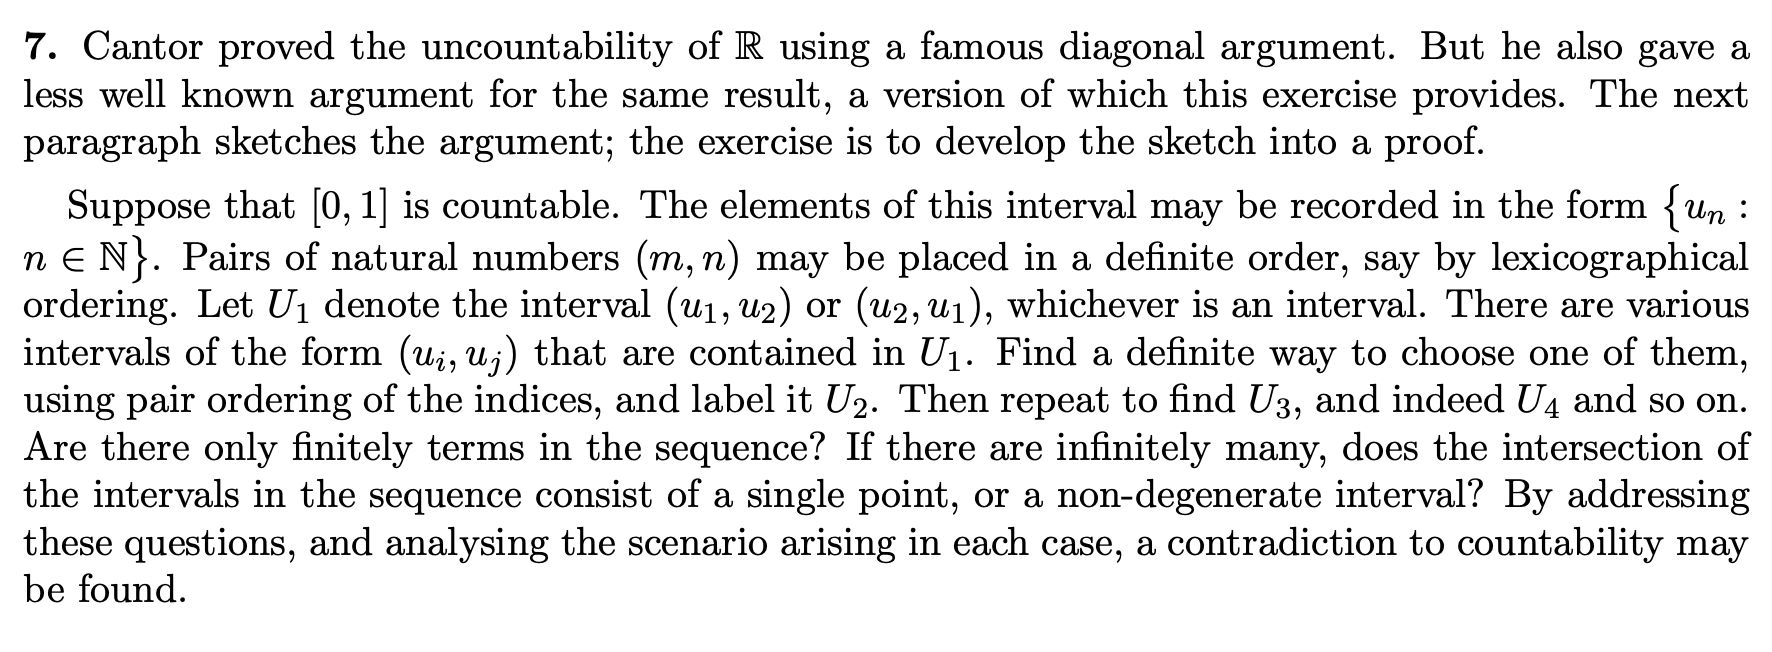
\includegraphics[width=400pt]{img/analysis--berkeley-202a--homework-1-a577.png}
\end{mdframed}


\begin{proof}
  Suppose for a contradiction that $[0, 1] \subset \R$ is countable. Fix an enumeration $\{u_n ~|~ n \in \N\}$
  of the elements of $[0, 1]$. (Note that the elements in the enumeration cannot be assumed to be in order: we
  are supposing countability of the reals, and it is an axiom that we can determine which is the greater of any
  two reals, but to enumerate them in order would require a successor function on the reals and we have not
  assumed we have that.)

  Our aim is to exhibit an element of $[0, 1]$ that is not present in the enumeration$\{u_n ~|~ n \in \N\}$.

  Pick two distinct elements from $[0, 1]$. Label the smaller $u_1$ and the larger $u_2$. Set $U_1 = [u_1, u_2]$.

  {\it Find a definite way to choose an interval in [u1, u2]:}
  \begin{enumerate}
  \item Set the lower limit of the interval to $u_1$, and for the upper limit, walk along the enumeration until we
    encounter the first one whose associated real is $< u_2$.
  \end{enumerate}



\end{proof}


\begin{proof}
  Suppose for a contradiction that $[0, 1] \subset \R$ is countable. This means that the elements of $[0, 1]$
  may be enumerated as $\{u_n ~|~ n \in \N\}$. Let $a = \min\{u_1, u_2\}$ and $b = \max\{u_1, u_2\}$. But
  then $\frac{a + b}{2}$ is a real number greater than $u_1$ and less than $u_2$ and therefore is missing from
  our original enumeration. Therefore no such enumeration exists.

  \red{NOPE: I think the problem here is you can't ``sort​'' a countably infinite set so you don't know that there is no other element between u1 and u2.}

\end{proof}




\begin{lemma}[Countable intersection of intervals yields a singleton]
  Let $x \in \R$. Then
      \begin{align*}
      \bigcap_{n=1}^\infty \Big(x -\frac{1}{n}, x\Big] = \{x\}.
    \end{align*}
\end{lemma}

\begin{proof}
  Recall that the notation $\bigcap_{n=1}^\infty f(n)$ means $\lim_{N\to\infty} \bigcap_{n=1}^N f(n)$. We have
  \begin{align*}
      \bigcap_{n=1}^\infty \(x -\frac{1}{n}, x\)
    &= \lim_{N \to \infty} \bigcap_{n=1}^N \(x -\frac{1}{n}, x\) \\
    &=
    \end{align*}
\end{proof}



\begin{proof}
  Suppose for a contradiction that $[0, 1] \subset \R$ is countable. This means that the elements of $[0, 1]$
  may be enumerated as $\{u_n ~|~ n \in \N\}$. We want to exhibit an element of $[0, 1]$ that is not present in
  such an enumeration.

 Let
  \begin{align*}
    U_1 &=
    \begin{cases}
      \big(u_1, u_2\big] ~~~~~~~\text{if } u_1 \leq u_2\\
      \big(u_2, u_1\big] ~~~~~~~\text{otherwise},
    \end{cases}\\
    U_2 &=
    \begin{cases}
      \big(u_1, \frac{1}{2}u_1 + \frac{1}{2}u_2\big] ~~~~~~~\text{if } u_1 \leq u_2\\
      \big(u_2, \frac{1}{2}u_2 + \frac{1}{2}u_1\big] ~~~~~~~\text{otherwise},
    \end{cases}\\
    U_3 &=
    \begin{cases}
      \big(u_1, \frac{2}{3}u_1 + \frac{1}{3}u_2\big] ~~~~~~~\text{if } u_1 \leq u_2\\
      \big(u_2, \frac{2}{3}u_2 + \frac{1}{3}u_1\big] ~~~~~~~\text{otherwise},
    \end{cases}\\
    \ldots,
  \end{align*}
  so that in general
  \begin{align*}
    U_k &=
    \begin{cases}
      \big(u_1, \frac{k-1}{k}u_1 + \frac{1}{k}u_2\big] ~~~~~~~\text{if } u_1 \leq u_2\\
      \big(u_2, \frac{k-1}{k}u_2 + \frac{1}{k}u_1\big] ~~~~~~~\text{otherwise}.
    \end{cases}
  \end{align*}




  Billingsley p.19:
  \begin{quote}
    ...require a collection that contains the intervals and is closed under countable unions and intersections.
    Note that a singleton $\{x\}$ is a countable intersection of intervals:
    \begin{align*}
      \bigcap_{n=1}^\infty \Big(x -\frac{1}{n}, x\Big] = \{x\}.
    \end{align*}
  \end{quote}



\end{proof}